\section{Manufacture Process}
This section will describe the full process of developing the step up converter PCB\@. That is simulation, PCB layout, and printing.\
\subsection{Design and simulation}
Firstly, simulations were made to experimentally come up with a theoretical solution to the problem. In this stage, total freedom was at hand which made the ability of finding errors and differentiate good solutions from bad ones simpler. The simulations were made in Multisim using the build in function generator and multimeter to measure the outcome. When the desired function had been simulated and verifired, the netlist, which is a description of the connectivity of the circuit, was carefully verified to maintain the desired function going into Ultiboard.
\subsection{PCB layout}
The Multisim file was transfered to Ultiboard where the last design choices were to be made. In Ultiboard, two crucial files were constructed.

The first one \textit{''Copper Top''}, which contains the information of where the printer shall print the silver traces, connecting all the components. Thanks to the netlist from Multisim, Ultiboard automatically connects all components making the process significantly easier. The components were placed as compact as possible, with simplicity in mind, see Fig.\ref{fig:PCB}. Next trace width and trace clearence was chosen to handle the voltage, current and frequency the circuit was designed for.

The next file \textit{''Solder Mask Top''}, contains information about where the printer shall print the soldering masks that the physical components later can be placed and soldered on to. This information is automatically generated from the footprints of the components, being chosen in the Multisim file.
\subsection{Printing}
After connecting the Voltera printer to the computer, the gerber file \textit{''Copper Top''} form Ultiboard was exported to the Voltera software to begin the printing process. The conductive ink \textit{''LaughingBear''} was used as the conductive trace material. The printer flow was calibrated to ensure good quality traces and pads with neither too much flow, resulting in possible shorts, nor too less, resulting in possible broken traces. The traces were printed and inspected to watch for possible faults. The board was then baked for about 30 minutes, using the ink specific, Voltera baking program, to harden the printed silver ink.

After the baking, the next gerber file \textit{''Solder Mask Top''} was loaded to begin the second printing phase. Here, the solder paste \textit{''FuriousAnt''} was used for the solder masks. The solder masks were printed and inspected to watch for possible shorts.

With solder paste on the pads, the components were ready to be placed on the board. A Small amount of extra solder paste was manually put on the pads of the pin strip footprint to strengthen the otherwise delicate structure. All the components exept the pin strip were carefully placed on the board using the component placing machine. The pin strip was manually placed on the board. Then the board was reflow soldered using the Voltera reflow program, this again took about 30 minutes.
\begin{figure}[h]
    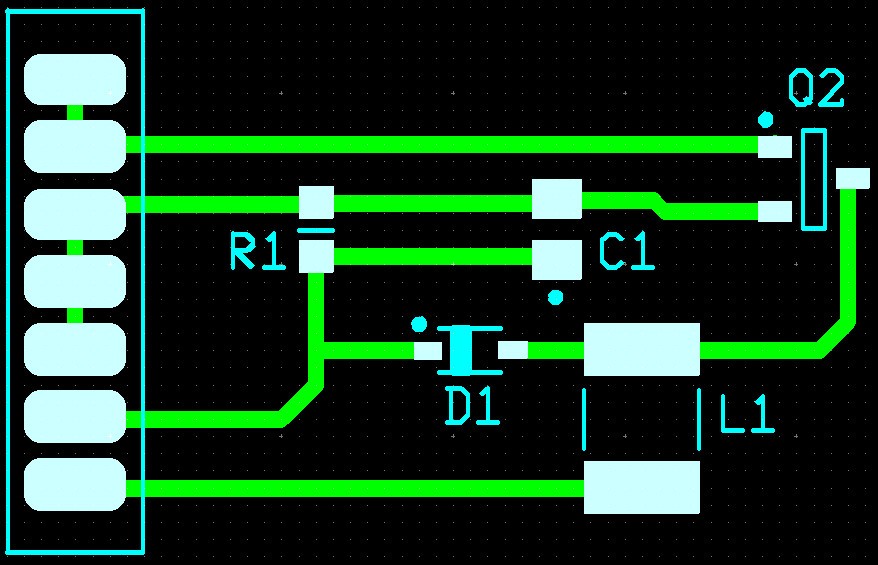
\includegraphics[width=\linewidth]{PCBlayout.jpg}
    \caption{Picture of the layout of the components on the PCB\@. R1\hyp{}resitor, D1\hyp{}diode, C1\hyp{}capacitor, L1\hyp{}inductor, Q2\hyp{}mosfet.}
    \label{fig:PCB}
\end{figure}
